\chapter{Introduction}

The Prisoner's Dilemma(PD) is a well known example in Game Theory and in recent
years has become the gold standard of understanding evolution of
co-operative behaviour \parencite{Lorberbaum1994}. That is due to the PD's nature.
In the example of the Prisoner's Dilemma two criminals have been arrested and
interrogated, with no ways of communicating,by the police.
They are given only two choices, to either cooperate with each other or defect.
By rational selection the outcome of a single run PD will alway be to defect,even
if by cooperating they can achieve the maximum reward.

The years 1980-1981, aroused much interest on Game Theory and the PD due to the
work done by both Axelrod and Hamilton, proving that copperation dehaviour
can emerge from PD if


This nature of the
PD illustrates the problems of two individuals achieving cooperation and it has
became a well studied topic in many fields, such as biology, sociology, ecology
and phycology.\parencite{Nowak_&_May1992}.

The first steps of


This dissertation will be reviewing some of the work done in PD and
IPD tournaments, will go through their topologies and try to give some kind of
definition on the spatial structure of a tournament.Lastly it will present the
concept of teamwork in spatial tournaments.

\section{The Prisoner's Dilemma}
The PD was originally formulated by Merril M. Flood and Melvin Dresher,
who were working on the Flood-Desher Experiment at the RAND cooperation in 1950.
Later in 1950, the mathematician Albert W. Tucker presented the first formal
representation of the PD, titled \"A Two-Person Dilemma\" in a seminar at
Stanford University\parencite{Gass2005}.

A description of the PD, found in \parencite{Li2011} is as follows :
There are two players that simultaneously have to decide to whether Cooperate(C)
or Defect (D) with each other, without exchanging informations.

\begin{itemize}
  \item If both players choose to cooperate they will both receive a reward (R)
  \item If a player defects and the other cooperates then the defector receives
  a temptation payoff (T) and the cooperator a sucker payoff (S)
  \item If both players defect they will both receive a penalty (P)
\end{itemize}

Fig. 1 illustrates the payoffs matrix.~\ref{fig:pd_payoff}.

\begin{figure}[h!]
\centering
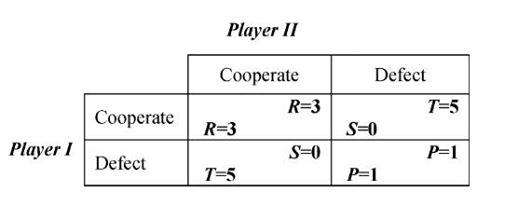
\includegraphics[scale=0.6]{pd_payoff.jpg}
\caption{Prisoner's Dilemma Payoff Matrix.\parencite{Li2011}}
\label{fig:pd_payoff}
\end{figure}

It can be shown that in the standar form of the PD a pure Nash Equilibrium exists
when both players defect. So the outcome of any one round game will be Defection.

The Prisoner’s Dilemma can also be studied for any given number of interations (IPD)
, where players play each other repeatedly. An extra condition for the payoffs
in the IPD are : T \(>\) R \(>\) P \(>\) S and R \(>\) 1/2(T+S).

\section{Tournaments}

In 1980-81, Robert Axelrod conducted a computer tournement where different
strategies for the Iterated Prisoner's Dilemma(IPD) clashed and a winner was annouched.
With 13 and 62 strategies respectively both tournaments shared the same topology
(round robin) and the same winner, which was Tit for Tat.
Moreover, Axelrod proved that cooperative behaviour emerging
depends on the probability of two players meeting  again.


Axelrod began an age of Game Theory and computer programming.
After his work various research was conducted trying to sight some light on the
cooperation evolution in IPD.

\section{Topologies}

Nowak and May, 1992, conducted their own experiment but this
time using a different topology that Axelrod. Instead of all the players playing
each other, this time the players would be represented in a lattice and they would
only play their neighbors.

After Nowak many other reserachers experimented with the spatial structure and
most of them used a 2D sqare lattice. Differences can be found between using
the PD or the IPD and whether there was evolution in their tournaments.

\section{Referencing}
We can make make in text citations automatically.
In the `author-year' style we can do this as:
\begin{itemize}
    \item A noun e.g. \textcite{Gillard2014}
    \item In parentheses e.g. \parencite{Gillard2014}
\end{itemize}

\section{Tables}
We can make nicer looking tables in \LaTeX~ using the `booktabs' package.
An example of this can be seen in Table.~\ref{fig:exampletable}.
\begin{table}[h]
\centering
\caption{An example table using the `booktabs' package}
\label{fig:exampletable}
\begin{tabular}{cccccccccc}
\toprule
& \multicolumn{3}{c}{\textbf{ABC}} & \multicolumn{3}{c}{\textbf{ABC}} & \multicolumn{3}{c}{\textbf{ABC}} \\
\cmidrule(lr){2-4}\cmidrule(lr){5-7}\cmidrule(lr){8-10}
\textbf{Example}      & \textbf{A}       & \textbf{B}       & \textbf{C}      & \textbf{A}           & \textbf{B}           & \textbf{C}          & \textbf{A}           & \textbf{B}           & \textbf{C}          \\
\cmidrule(lr){1-1}\cmidrule(lr){2-4}\cmidrule(lr){5-7}\cmidrule(lr){8-10}
0         & 1234      & 1234     & 1234     & 1234          & 1234         & 1234         & 1234        & 1234         & 1234         \\
1         & 1234      & 1234     & 1234     & 1234          & 1234         & 1234         & 1234          & 1234         & 1234         \\
2         & 1234      & 1234     & 1234     & 1234          & 1234         & 1234         & 1234        & 1234         & 1234        \\
3         & 1234      & 1234     & 1234     & 1234          & 1234         & 1234         & 1234        & 1234         & 1234         \\ \bottomrule
\end{tabular}
\end{table}

\section{Footnotes}
We can make footnotes\footnote{This is a footnote} easily.

\section{Sub-figures}
Using the subcaption package we can make side by side figures.
For example see Fig.~\ref{fig:subfigureexample}.

\begin{figure}[h]
\centering
    \begin{subfigure}[t]{0.45\textwidth}
    \centering
        
\includegraphics[width=\linewidth]{image1.png}
    \caption{First sub-figure}
    \end{subfigure}
\hfill
    \begin{subfigure}[t]{0.45\textwidth}\centering
    \centering
        
\includegraphics[width=\linewidth]{image1.png}
    \caption{Second sub-figure}
    \end{subfigure}
~
\caption{Example of using subfigures}
\label{fig:subfigureexample}
\end{figure}
